% vim: set spelllang=fr:
\pagestyle{empty}
\cleardoublepage

\setlength{\oddsidemargin}{79pt}
\setlength{\marginparsep}{0pt}
\setlength{\marginparwidth}{0pt}
\setlength{\marginparpush}{0pt}
\setlength{\hsize}{\paperwidth}
\addtolength{\hsize}{-\oddsidemargin}
\addtolength{\hsize}{-\oddsidemargin}
\addtolength{\hsize}{-2in}

\begin{center}
\begin{minipage}{.6\textwidth}
\centering
{\Large Crédits illustrations}

\vspace{1.5cm}
Figures \ref{sa:fig:gspnex1} à\textit{/to} \ref{sa:fig:lha}:\\
Paolo \textsc{Ballarini}\quad(©~2011)
\medskip

Figures \ref{tj:fig:zerotest} à\textit{/to} \ref{tj:fig:memory42}:\\
Mathieu \textsc{Sassolas}\quad(©~2014)

\bigskip
Ces illustrations sont soumises au droit d'auteur de leur créateur respectif.

\medskip
\textit{Those illustrations are subject to the copyright of their respective author.}
\end{minipage}
\end{center}

\vfill

\begin{small}
Le terme «Bluetooth» est une marque déposée du \textit{Bluetooth Special Interest Group}.
Le terme «grsecurity» est une marque déposée de l'\textit{Open Source Security, Inc}.
Les termes «IEEE», «802», «IEEE~802.11», «IEEE~802.15.1» et «IEEE~802.15.4» sont des marques déposées de l'\textit{Institute of Electrical and Electronics Engineers}.
Le terme «Linux» est une marque déposée au nom de Linus \textsc{Torvald}.
Le terme Wi-Fi est une marque déposée de la \textit{Wi-Fi Alliance}.
Le terme ZigBee est une marque déposée de la \textit{ZigBee Alliance}.
\medskip

{\it
“Bluetooth” is a trademark of the Bluetooth Special Interest Group.
“grsecurity” is a trademark of the Open Source Security, Inc.
“IEEE”, “802”, “IEEE~802.11”, “IEEE~802.15.1” and “IEEE~802.15.4” are trademarks of the Institute of Electrical and Electronics Engineers.
“Linux” is a trademark of Linus \textsc{Torvald}.
“Wi-Fi” is a trademark of the Wi-Fi Alliance.
“ZigBee” is a trademark of the ZigBee Alliance.
}
\end{small}

\vfill

%\begin{center}
%\begin{minipage}{.6\textwidth}
%\centering
%\href{https://creativecommons.org/licenses/by/4.0/deed.fr}{\includegraphics{Back/by.eps}}

%\bigskip
%Le reste de cet ouvrage est mis à disposition selon les termes de la
%\href{https://creativecommons.org/licenses/by/4.0/deed.fr}{licence Creative Commons Attribution 4.0 International}.

%\medskip
%\textit{The remainder of this work is licenced under a
%\href{https://creativecommons.org/licenses/by/4.0}{Creative Commons Attribution 4.0 International License}.}
%\end{minipage}
%\end{center}
\begin{center}
\begin{minipage}{.6\textwidth}
\centering
\href{https://creativecommons.org/publicdomain/zero/1.0/deed.fr}{
\includegraphics[width=3cm]{Back/cc-zero.eps}}

\bigskip
Le reste de cet ouvrage est mis à disposition\\selon les termes de la\\
\href{https://creativecommons.org/publicdomain/zero/1.0/deed.fr}{licence universelle Creative Commons Zéro 1.0}\\(transfert dans le domaine public).

\medskip
\textit{The remainder of this work is licenced under a\\
\href{https://creativecommons.org/publicdomain/zero/1.0}{Creative Commons Zero 1.0 Universal License}\\(Public Domain Dedication).}
\end{minipage}
\end{center}

\cleardoublepage
\mbox{}\vfill
\newcommand\figrefdcloud  { -- \ref{in:fig:cloud}}
\newcommand\figrefdia     { -- \ref{st:fig:wsnintro}, \ref{st:fig:wsn}, \ref{sa:fig:network}, \ref{sa:fig:detection}, \ref{sa:fig:elecself}, \ref{sa:fig:elecch}, \ref{sa:fig:elecbs}, \ref{se:fig:vnodes}}
\newcommand\figrefgnuplot { -- \ref{sa:fig:detec-nbcn}, \ref{sa:fig:detection-txRate}, \ref{sa:fig:conso-moyenne}, \ref{sa:fig:conso-ecart-type}, \ref{sa:fig:premier-deces}, \ref{sa:fig:capteurs-en-vie}, \ref{sa:fig:detection-dos}, \ref{se:fig:mean}, \ref{se:fig:overhead}, \ref{se:fig:stddev}, \ref{sd:fig:cons-inf}, \ref{sd:fig:cons-inf-zoom}, \ref{sd:fig:stddev-inf}, \ref{sd:fig:nbnodes-10J}, \ref{sd:fig:nbnodes-20J}, \ref{sd:fig:detec-one-10J}, \ref{sd:fig:detec-min-10J}, \ref{sd:fig:detec-min-20J}}
\newcommand\figrefgraphviz{ -- \ref{se:fig:states}}
\newcommand\figrefinkscape{ -- \ref{sa:fig:grille}, \ref{sa:fig:gspnex1}, \ref{sa:fig:snodegspn}, \ref{sa:fig:chgspn}, \ref{sa:fig:cnodegspn1}, \ref{sa:fig:cnodegspn2}, \ref{sa:fig:petricluster}, \ref{sa:fig:petridyn}, \ref{sa:fig:petrielec}, \ref{se:fig:states}, \ref{se:fig:cover}, \ref{sd:fig:neighbors}, \ref{sd:fig:star}}
\newcommand\figreftex     { -- \ref{st:fig:sensor}, \ref{st:fig:tcpip}, \ref{ea:fig:tcpip}, \ref{ea:fig:idsmap}, \ref{sa:fig:eqtrans}, \ref{sa:fig:lha}, \ref{tj:fig:autGoodNode}, \ref{tj:fig:autBadNode}, \ref{tj:fig:autFirstTurn}, \ref{tj:fig:zerotest}, \ref{tj:fig:halt}, \ref{tj:fig:infmemoryneeded}, \ref{tj:fig:memory42}}

\begin{center}
    \noindent Cet ouvrage a été entièrement conçu et réalisé à l'aide\\des logiciels libres suivants:
    \bigskip

    \begin{tabu}to .6\linewidth {c X[4,l]}
        \href{http://biblatex-biber.sourceforge.net}{\textsf{biber}}                                  & (bibliographie) \\
        \href{https://github.com/jasondavies/d3-cloud}{\textsf{d3-cloud}}                             & (illustration: nuage de mots\figrefdcloud) \\
        \href{https://wiki.gnome.org/Apps/Dia}{\textsf{Dia}}                                          & (illustrations\figrefdia) \\
        \href{http://git-scm.com}{\textsf{Git}}                                                       & (archivage des versions) \\
        \href{http://www.gnuplot.info}{\textsf{Gnuplot}}                                              & (illustrations: graphiques\figrefgnuplot) \\
        \href{http://www.graphviz.org}{\textsf{Graphviz}}                                              & (illustration: machine à états\figrefgraphviz) \\
        \href{https://inkscape.org}{\textsf{Inkscape}}                                                & (illustrations\figrefinkscape) \\
        %\href{http://www.isi.edu/nsnam/ns}{\textsf{ns-2}}, \href{https://www.nsnam.org}{\textsf{ns-3}} & (simulations) \\
        \href{http://www.vim.org}{\textsf{Vim}}                                                       & (édition) \\
        \href{https://code.google.com/p/waf}{\textsf{Waf}}                                            & (compilation) \\
        \href{http://xetex.sourceforge.net}{\XeTeX}                                                   & (mise en page, illustrations\figreftex)
    \end{tabu}
\end{center}
\vfill
\begin{center}
\href{http://www.orthographe-recommandee.info}{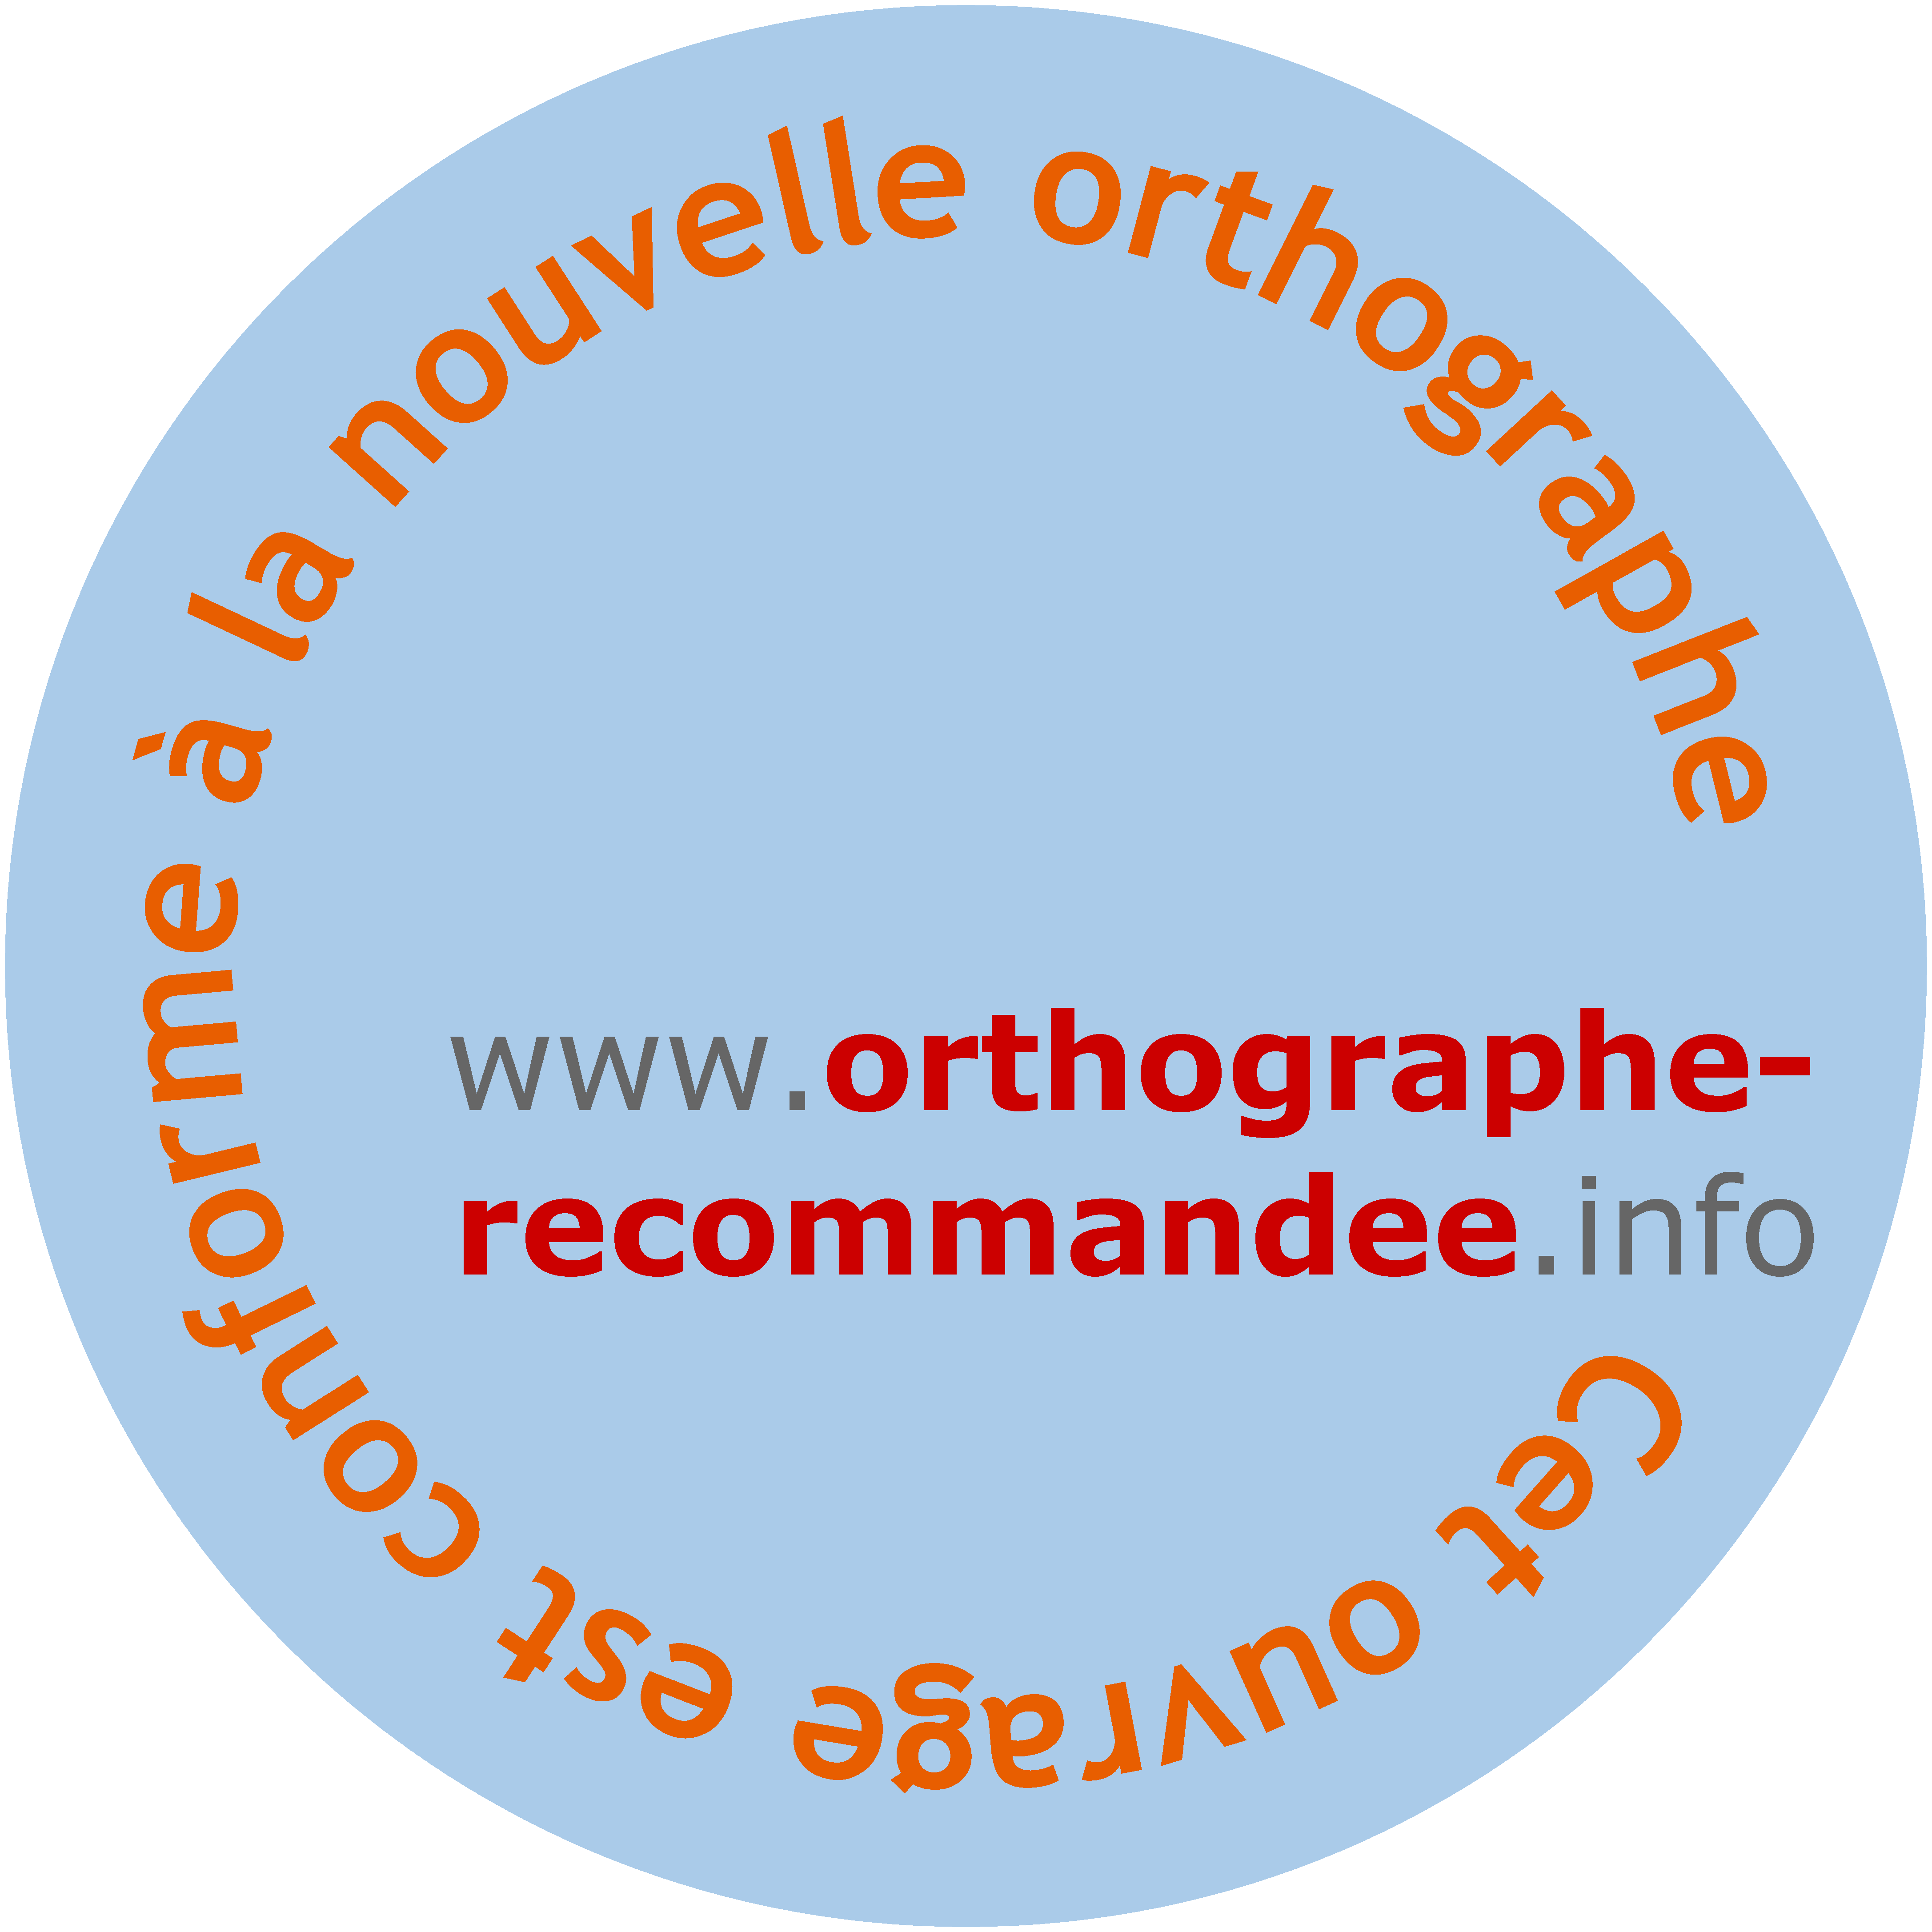
\includegraphics[width=3.5cm]{Back/ouvrage.pdf}}
\end{center}
\vfill
\begin{center}
Les fichiers sources utilisés pour réaliser cet ouvrage sont disponibles à l'adresse suivante:\\
\url{https://github.com/Qeole/PhD}
\end{center}
